\chapter{Pulitzer Prize-Winner Explains His Writing Process --- Richard Powers}

This lecture begins with a hard, compressed maxim and then spends the rest of its hour unfolding it. Character becomes visible under pressure; pressure becomes drama; drama widens from the inward life of a single person to the collisions among people and finally to the larger world in which those people live. From there the discussion descends into craft in the narrow sense: voice, diction, register, syntax, predication, surprise, revision, openings, dialogue, and the daily conditions under which sentences arrive. What follows is a companion text that keeps that order. We begin with pressure and collision, and only later do we ask how the words themselves make such pressure legible on the page.

\section{Character, Pressure, and the Three Levels of Drama}

Powers opens with a claim that is both moral and technical. We do not really know a character when everything is easy. We know a character when values collide and something must be lost. In this sense, drama is not a decorative addition to character; it is the condition under which character becomes visible.

A compact way to write the lecture's causal spine is
\begin{equation}
\text{character} \Rightarrow \text{drama}.
\end{equation}
This is not yet a theory of plot. It is a theory of pressure. If we press hard enough, a hierarchy of commitments appears. If we do not press, we may get traits, surfaces, and agreeable sketches, but not the thing itself.

Powers then scales the problem outward and gives us three kinds of collision:
\begin{equation}
\text{person vs self},\qquad \text{person vs person},\qquad \text{person vs world}.
\end{equation}
The first collision is interior. A person wants to keep two goods that cannot both be kept. The second is social and political. Two people, each rendered sympathetically, want incompatible outcomes. The third is larger still: human beings want to tell a certain story about what the good life is, but the world may be indifferent to that story or hostile to it.

Before he arrives at these formal levels, Powers motivates them by returning character to ordinary life. We are already constantly inferring motives, hidden resentments, regrets, nostalgias, and unrealized alternatives in the people around us. We are, as he puts it, novelists in our own lives. Fiction does not invent that faculty from nothing; it disciplines and extends it.

\subsection{Question \& Answer}

\paragraph{Question.} Where does drama actually come from?

\paragraph{Answer.} It comes from collision, and collision becomes visible only under pressure. A value conflicts with another value, a person conflicts with another person, or a human project conflicts with the larger world. The lecture's first cold-open phrase, ``push them to the wall,'' is therefore not rhetoric but method. It tells us how to move from a merely described person to a dramatic person.

\section{The Onion of Character: Traits, Mannerisms, and Core Inner Values}

Having established that character becomes visible under pressure, Powers asks how we build character before pressure arrives. His teaching image is the onion. Outwardly we see traits; beneath traits we find mannerisms; beneath mannerisms we find core inner values.

We may summarize the model schematically as
\begin{equation}
\text{core inner values} \to \text{mannerisms} \to \text{traits}.
\end{equation}

\begin{figure}[h]
\centering
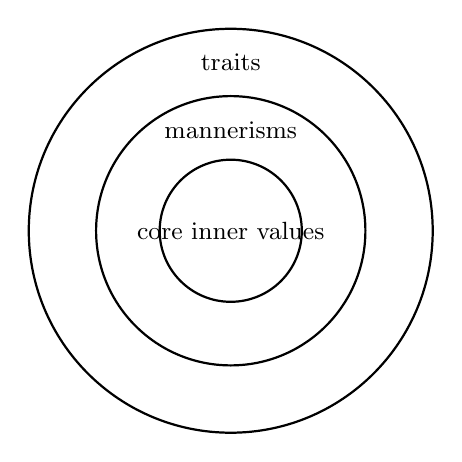
\begin{tikzpicture}[scale=0.95]
\draw[thick] (0,0) circle (2.7);
\draw[thick] (0,0) circle (1.8);
\draw[thick] (0,0) circle (0.95);
\node at (0,2.25) {\small traits};
\node at (0,1.35) {\small mannerisms};
\node at (0,0) {\small core inner values};
\end{tikzpicture}
\caption{A schematic reconstruction of Powers's ``onion'' model of character.}
\end{figure}

Traits are the outer shell: clothing, posture, haircut, visible habits, small performative details by which a reader first sees a person. But Powers is careful here. These are not the person. They are manifestations. A trait comes from somewhere. Beneath it lies a mannerism: a recurrent way of behaving, speaking, deflecting, soothing, needling, or performing selfhood. Beneath that mannerism lies a value. A person may habitually set others at ease because he values complicity, attentiveness, loyalty, or some other inward commitment.

At this point the lecture adds a useful complication. The arrows in the onion are not one-to-one. Multiple values may underwrite the same mannerism, and multiple mannerisms may support the same visible trait. Character is therefore not solved by labeling. It is solved by coherence: the outer behavior must both reveal and conceal what the person is trying to preserve.

This is where pressure re-enters. If a character values honesty and fidelity, then these values remain static abstractions until we place them in a circumstance where both cannot survive together. The lecture's example is blunt and effective:
\begin{equation}
\text{honesty} + \text{fidelity} + \text{forced choice} \Rightarrow \text{interior drama}.
\end{equation}
A friend has done something wrong. Do we expose him and preserve honesty, or protect him and preserve fidelity? The story appears precisely where preservation becomes impossible.

\subsection{Question \& Answer}

\paragraph{Question.} How do we turn a person into a dramatic character rather than a mere description?

\paragraph{Answer.} We move inward before we move outward. We begin with traits, infer mannerisms, infer the values behind those mannerisms, and then force those values into conflict. The description becomes a character only when something essential is at risk.

\section{Beyond the Human World: Ecological and Metaphysical Drama}

Once the inner and interpersonal scales are in place, Powers widens the frame. There is a third kind of drama, and modern literary fiction, in his telling, often neglected it for a long time. We may formalize his widening of scale as
\begin{equation}
\text{psychological} \to \text{sociological/political} \to \text{environmental/metaphysical}.
\end{equation}

The point is not ornamental. Human beings want to have a project in the world. They have a picture of the good life. But the world is not merely scenery surrounding that picture. It may resist it. In that sense, the third drama is not a subclass of setting; it is a clash between human desire and planetary circumstance.

Powers then historicizes the claim. He suggests that much literary fiction became extremely capable in its treatment of psychology and sociology while often treating human beings as though they were autonomous from everything else. The older ``man against nature'' story came to seem quaint, nostalgic, or second-class. Yet in recent decades, as ecological crisis returns to consciousness, that third drama floods back into serious fiction.

The lecture turns here toward \emph{The Overstory}, but the key point is broader than one novel. Attention to the nonhuman world is not a side excursion away from character. It is another route into character. Powers explicitly says that to look at the nonhuman world is also to understand interior drama. Old mythic and indigenous literatures knew this already. So did childhood. The young child is an animist not because the child is foolish, but because the child has not yet lost the instinct that aliveness exceeds the human.

The lecture's fusion is therefore not ``science versus spirit'' but a more difficult conjunction. One must know the world as a scientist knows it, and also as an animist or pantheist child knows it. That dual knowledge is not a contradiction but a widening of available reality.

\subsection{Question \& Answer}

\paragraph{Question.} Why must stories move beyond the human if they are to capture the full scale of drama?

\paragraph{Answer.} Because human life is not self-enclosed. A person does not only collide with private desire and other people. A person also collides with the terms set by the larger world. If fiction omits that dimension, it narrows the field of conflict and mistakes the whole for a part.

\section{Why Fiction Moves Us: Story, Affect, and Value Change}

The lecture now makes a decisive turn. Why does any of this matter? Why not simply state the facts, give the argument, and be done? Powers answers by distinguishing two things that are often confused:
\begin{equation}
\text{apprehension of fact} \neq \text{shift in values}.
\end{equation}
We may know something and still fail to live differently because of it. We may intellectually understand the ecology of a forest and still not feel our commitments move.

Powers's answer is that fiction works by a different path:
\begin{equation}
\text{story} \Rightarrow \text{affect} \Rightarrow \text{identification} \Rightarrow \text{movement of the reader}.
\end{equation}
The etymological aside on emotion matters here. Emotion is not merely a private feeling-state; it is, in a very old sense, movement. A story moves us. It relocates us within another person's predicament. It asks, ``Who would I be if I were not myself but that person?''

The lecture supports this claim with a concrete experimental pattern. One group reads neutral material, another reads information, another reads a moving fictional narrative. Afterwards, the apparently unrelated chance to help a stranger is staged. Those who have just been induced into affective identification are more likely to help. The point is not that fiction magically improves human beings forever. The point is that identification alters the immediate baseline from which action proceeds.

\paragraph{Worked example.} The logic of the experiment can be written as a short derivation:
\begin{enumerate}
\item A reader encounters a narrative rather than bare data.
\item The narrative recruits affect.
\item Affect recruits identification with another person.
\item Identification temporarily increases empathy.
\item Increased empathy changes what the reader is moved to do.
\end{enumerate}
This is exactly the distinction Powers wants us to keep in view. Statistics and arguments may sharpen apprehension. Story may shift value.

\subsection{Question \& Answer}

\paragraph{Question.} Why can a story move a reader when an argument cannot?

\paragraph{Answer.} Because story changes the route by which the material arrives. Argument addresses assent; story recruits identification. Once the reader begins to inhabit another perspective, the resulting movement is not merely conceptual. It can become behavioral.

\section{Voice from Below: Register, Diction, Syntax, and Predication}

Only after establishing what fiction does does Powers ask how it does it. He returns to the lecture's causal chain and tightens it:
\begin{equation}
\text{voice} \Rightarrow \text{character}, \qquad
\text{diction/register/syntax} \Rightarrow \text{voice}.
\end{equation}
A fuller schematic form is
\begin{equation}
\text{diction/register/syntax} \Rightarrow \text{voice} \Rightarrow \text{character} \Rightarrow \text{drama} \Rightarrow \text{form}.
\end{equation}

At the lowest level lie words and their social coloring. Register is the level of speech: casual, formal, slangy, ceremonious, intimate, stiff. Powers uses simple imperatives to show how much is carried by word choice alone. ``Hand me that,'' ``give me that,'' ``would you please pass that,'' and a mere ``yo'' followed by a gesture all request approximately the same outcome, but each performs a different relation between speaker and listener.

He then adds a historical layer. English contains a kind of built-in bilingualism, especially between Anglo-Saxon and Latinate vocabularies. That difference does not merely vary sound; it varies social register. ``House'' and ``mansion,'' ``freedom'' and ``liberty,'' do not only denote. They color, stratify, and signal.

But diction is not enough. Powers wants a tractable grammar lesson, and so he reduces the sentence to its kernel.

\begin{definition}
By \emph{predication} Powers means the main subject together with the main verb. This is the heart of the sentence, the structure around which the rest is arranged.
\end{definition}

We may write this as
\begin{equation}
\text{predication} = \text{main subject} + \text{main verb}.
\end{equation}

From this definition Powers derives three sentence species:
\begin{equation}
SV\cdots,\qquad \cdots SV,\qquad S\cdots V.
\end{equation}
The notation is schematic, but the insight is precise. We can front-load the predication, delay it, or split it. These are not merely grammatical alternatives. They are ways of reproducing states of mind in the reader.

\paragraph{Worked example.} Powers's two clearest examples can be aligned as follows:
\begin{align}
\text{``He pointed the gun at his friend.''} &\sim SV\cdots,\\
\text{``Way back across the yard, near the fence, \dots she hid.''} &\sim \cdots SV.
\end{align}
In the first case, the action arrives immediately; the sentence shocks up front and lets the consequences trail after. In the second case, modifiers postpone the kernel, and the reader waits in suspense for the hidden subject and verb. The sentence hides the woman in grammar before the scene hides her in space.

The split form, $S\cdots V$, is the rarest and Powers treats it more cautiously. The subject appears, material intervenes, and the verb arrives late. This may create suspense, comedy, or a kind of tonal key-change. But the larger point is already clear: sentence shape itself can participate in the affect of what is being described.

\subsection{Question \& Answer}

\paragraph{Question.} What drives voice if voice drives character?

\paragraph{Answer.} Words drive voice, but not words alone. Register, diction, syntax, cadence, and the placement of predication all contribute. Voice is the effect we hear when these choices align; character is what we infer from that heard performance.

\section{Description, Expectation, and Revision}

Powers now moves from sentence architecture to the local music of description. His example is memorable because it does several things at once: ``Each child's tree has its own excellence.'' The descriptive catalogue that follows makes species distinct, but the first sentence matters even more. Why ``excellence''? Why at the end?

Here the lecture introduces a readerly model of expectation. As we read, we forecast continuations. In a compact editorial shorthand, the idea may be expressed as
\begin{equation}
P(w_{n+1}\mid w_1,\dots,w_n),
\end{equation}
though Powers himself states the point informally: we are always asking what comes next. The beginning and end of the sentence are therefore high-voltage locations.

What happens in the tree sentence is that the reader's expectation is lightly bent. An ordinary continuation might have preserved the music of the line while ending on something flatter. ``Excellence'' arrives instead and changes the color. The sentence finishes in a key we did not quite predict. The surprise is not wild; it is controlled. Powers's claim is that such control creates a small but real rise in tension.

We may summarize the mechanism like this:
\begin{equation}
\text{expected ending} \Longrightarrow \text{surprising but apt ending} \Longrightarrow \text{local increase in tension}.
\end{equation}

The second major claim in this section concerns revision. The first draft is not condemned because it tries too hard. Often it must try too hard. One may have to make the effect visible to oneself before one can hide the footwork. Revision is then not a separate bureaucratic phase but the continuation of perception. The writer returns to the sentence, hears where it overstates, and tunes it again.

Powers is emphatic here: there is no final right. The writer moves, the reader moves, the world moves. One hears an old sentence years later and wants to revise it again. This should not be mistaken for failure. It is the signature of a living art.

\subsection{Question \& Answer}

\paragraph{Question.} How do we write vividly without sounding overwritten?

\paragraph{Answer.} First we allow ourselves to overstate the intention in draft. Then we revise toward precision, concealment, and musical control. Vividness does not come from piling on description. It comes from choosing the one detail, the one word, or the one turn of syntax that reorients the reader's attention.

\section{Openings, Tension Graphs, Dialogue, and the Writing Life}

Powers's discussion of openings is continuous with everything that came before. An opening line is not an isolated ornament. It is a compressed version of the book's tensions and scale. His own openings often begin cosmically and then descend toward the local, as if the ear wanted a wide establishing shot before allowing the close-up. One earns the right to tell a local story by first showing the size of the canvas.

This leads naturally to the lecture's large-scale account of form. If drama is collision, then the primary variable across a book is tension.

\begin{definition}
Tension is the reader's and the protagonists' realization that the stakes are going up.
\end{definition}

The lecture's structural sequence is
\begin{equation}
\text{hook} \to \text{exposition} \to \text{rising action} \to \text{climax},
\end{equation}
and with the after-stage included,
\begin{equation}
\text{hook} \to \text{exposition} \to \text{rising action} \to \text{climax} \to \text{denouement}.
\end{equation}
The crucial recursive engine is
\begin{equation}
\text{solve local instability} \Rightarrow \text{larger instability}.
\end{equation}
If one simply stacks bigger and bigger dragons in a straight line, the pattern becomes mechanical. The art lies in sculpting the graph: a hook that starts slightly above resting level, an exposition that relaxes without losing curiosity, a middle in which every resolution enlarges consequences, a climax where stakes cannot rise further, and a denouement in which the knot blows apart and consequences re-enter the world.

\begin{figure}[h]
\centering
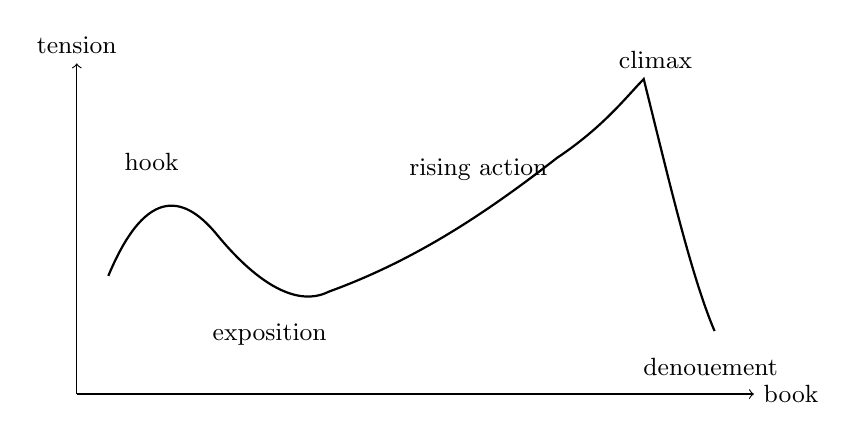
\begin{tikzpicture}[x=1cm,y=1cm]
\draw[->] (0,0) -- (8.6,0) node[right] {\small book};
\draw[->] (0,0) -- (0,4.2) node[above] {\small tension};
\draw[thick] (0.4,1.5)
  .. controls (0.9,2.7) and (1.4,2.5) .. (1.8,2.0)
  .. controls (2.3,1.4) and (2.8,1.1) .. (3.2,1.3)
  .. controls (4.3,1.7) and (5.2,2.3) .. (6.1,3.0)
  .. controls (6.7,3.4) and (7.0,3.8) .. (7.2,4.0)
  .. controls (7.5,2.8) and (7.8,1.5) .. (8.1,0.8);
\node at (0.95,2.95) {\small hook};
\node at (2.45,0.75) {\small exposition};
\node at (5.1,2.85) {\small rising action};
\node at (7.35,4.25) {\small climax};
\node at (8.05,0.35) {\small denouement};
\end{tikzpicture}
\caption{A schematic reconstruction of Powers's long-form tension graph.}
\end{figure}

\subsection{Question \& Answer}

\paragraph{Question.} How does drama generate structure over the length of a whole book?

\paragraph{Answer.} Because tension is not local only. The same collisions that animate the scene also determine the book's global shape. A hook raises immediate interest, exposition locates the players, rising action enlarges instability, climax forces the final jump, and denouement releases consequence back into the world.

After this, the lecture returns from structure to practice. Dialogue, Powers says, is not empirically exact speech. Real conversation transcribed verbatim would often be chaos. Good dialogue is stylized speech that knows the conventions of plausibility at a given cultural moment. Its test is not stenographic accuracy but vitality. This is why Powers insists on hearing dialogue aloud. Readers subvocalize; the writer should too.

The closing pages of the lecture widen once more, now toward the life of the writer. Solitude matters, but not as permanent withdrawal. One moves into solitude to generate traction and out of solitude to test the work against the world. The earlier discipline was numerical:
\begin{equation}
1000\ \text{words/day}.
\end{equation}
Later, that quota gives way to a different accountability: attention to the living world, walks, weather, landscape, presence, the nonhuman. Sentences now arise less from coercion than from renewed contact.

A fair schematic summary of this late process is
\begin{equation}
\text{solitude} \to \text{composition} \to \text{return to the world} \to \text{correction}.
\end{equation}
The lecture ends, then, where it began. Pressure matters, but so does replenishment. Structure matters, but so does aliveness. The writer alternates between narrowing the field enough to hear and widening it enough to tell the truth.

\section{Summary}

Powers's lecture gives us a connected sequence rather than a list of tips. Character becomes legible under pressure. Character under pressure generates drama. Drama widens from the inward to the interpersonal and then to the planetary. Fiction moves readers not merely by informing them but by recruiting affect and identification. Voice arises from word choice, register, syntax, and the placement of predication. Sentences create expectation and surprise; revision is the ongoing tuning of that expectation. On the scale of the whole book, drama becomes form through the management of tension. And at the scale of a life, writing becomes a repeated movement between solitude and the world, between construction and correction, between attention and form.